\documentclass{article}
\usepackage{graphicx}
\usepackage{hyperref}

\title{Assignment 2}
\author{Abbas Khan , Mariya Rybalka , Linara Adilova}
\begin{document}
\maketitle 
    
\section*{Task 2.1 (theoretical): glibc exploit}
    The vulnerability CVE- 2015-7547 was in glibc library. GNU C Library glibc, is a library of commonly-used functions for software written in the C language to run in Linux. Its "getaddrinfo()" function is used by the client side DNS resolver, a service that translates human-friendly websites names into computer-friendly network addresses.
\\
When making a DNS request, getaddrinfo() allocates 2048 bytes of memory for the answer, but does not check that the answer it receives fits in that buffer. The buffer overflow occurs in the function send{\_}dg (UDP) and send{\_}vc (TCP) for the NSS module libnss{\_}dns when calling getaddrinfo with AF{\_}UNSPEC family and in some cases also with AF{\_}INET6 before the fix in
commit 8479f23a.
\\
A malicious DNS server or a man-in-the-middle attacker could provide a DNS answer that is larger than 2048 bytes, overflowing the buffer and potentially allowing the attacker to execute malicious commands.
	  
\subsection*{NX(no execute)}
AMD's NX bit, which stands for no execute, is a technology used in CPU's to separate memory areas
for use by code and data.If the memory section has the NX attribute, this means that no processor instructions can be executed there.i.e An attacker who launches a buffer overflow attack to change
the "return address" to point to his malware code stored in the data area of the memory will be 
defeated by a set NX attribute on the respective memory because it will not allow code in the
memory area to be executed. 
	 
\subsection*{Address space layout randomization (ASLR)}
Address space layout randomization (ASLR) is a computer security technique involved in protection from buffer overflow attacks. In order to prevent an attacker from reliably jumping to, for example, a particular exploited function in memory, ASLR randomly arranges the address space positions of key data areas of a process, including the base of the executable and the positions of the stack, heap and libraries.i.e In case of buffer overflows the return addresses were overwritten with addresses that were known to be stable.
\\
However, when an application has ASLR enabled on its binary, attempts to redirect execution flow
into stack-based shellcode via a hard-coded address is likely to fail,because the location in 
memory of the stack buffer in question will be randomized, and guessing it would be potluck.

\section*{Task 2.2 (thoretical): Recent vulnerabilities, attacks or breaches }
DROWN: Breaking TLS using SSLv2, vulnerability CVE-2016-0800, presented in paper by Nimrod Aviram et al., at March 1, 2016.
\\
They presented a novel cross-protocol attack that allows an attacker to break a passively collected RSA key exchange for any TLS server if the RSA keys are also used for SSLv2, possibly on a different server. The name of the attack is DROWN - Decrypting RSA using Obsolete and Weakened eNcryption.
\\
In its general version, the attack exploits the protocol flaws in SSLv2, does not rely on any particular library implementation, and is feasible to carry out in practice for commonly supported export-grade ciphers. In order to decrypt one TLS session, the attacker must passively capture about 1,000 TLS sessions using RSA key exchange, make 40,000 SSLv2 connections to the victim server and perform $2^{50}$ symmetric encryption operations. 
\\
Authors found that 11.5 million (33\%) HTTPS servers are vulnerable to our attacks, because many HTTPS servers that do not directly offer SSLv2 share RSA keys with other services that do. Of servers offering HTTPS with browser-trusted certificates, 22\% are vulnerable.
\\
It might be, that all of us, using TLS connections, were affected by this attack. Also, for example BASIS University system also uses TLS connection, that might be connected with some SSLv2 server.
\\
The information and link to the article (https://drownattack.com/drown-attack-paper.pdf) was found on the Security Week site (http://www.securityweek.com). To me it seems to be reasonable to trust this source.

\section*{Task 2.3 (practical): Website Login credentials}
htpasswd is used to create and update the flat-files used to store usernames and password for basic authentication of HTTP users. htpasswd encrypts passwords using either bcrypt, a version of MD5 modified for Apache, SHA1, or the system's crypt() routine. Files managed by htpasswd may contain a mixture of different encoding types of passwords; some user records may have bcrypt or MD5-encrypted passwords while others in the same file may have passwords encrypted with crypt().
\\
The format of file is username:encrypted password.The result of MD5 encryption has following format:
"{\$}apr1{\$}" + the result of an Apache-specific algorithm using an iterated (1,000 times) MD5 digest of various combinations of a random 32-bit salt and the password. In our case the method of encryption used was MD5 as indicated by {\$}apr1{\$} at the start. The salt for an MD5 password is between {\$}apr1{\$} and the following {\$}. In our case the salt was "/pE9u4cQ". The validity of these conclusions could be easily checked by encrypting known password and checking the result. Than, having in mind, that the new password was taken from the specific text, one could just go word by word and encrypt every one of them and compare to the cypher in the file.

\section*{Task 2.4 (thoretical): Password Complexity}
\subsection*{a) Dictionary Attacks}
\begin{itemize}
\item RockYou is a company that developed widgets for MySpace and implemented applications for various social networks including Facebook. Since 2014, it has engaged primarily in the purchases of rights to classic video games, then incorporates in-game ads and re-distributes them.
\\
In December 2014, researchers at database security firm Imperva discovered the flaw in RockYou.com. But before RockYou could fix the bug, at least one hacker, using the alias "igigi", claims to have broken into the database and obtained the RockYou credentials of all users - totaling more than 32.6 million. He was able to steal the information because users' email addresses and passwords were stored in clear text, meaning they were not rendered unreadable through encryption or any other methods. Individuals must use their webmail address and password as their RockYou credentials to register for applications. The RockYou database was accessed through SQL injection, an attack process by which a hacker adds additional SQL code commands to a page request, and the web server then tries to execute those commands within the backend database. Vulnerable web applications process the extra SQL commands, which then causes the web application to leak additional information.
\\
Now this list of passwords is used as biggest available dictionary for checking the security of the passwords and for simple hack attacks. I think that companies concerned with security will be ensured, that the private information cannot be accessed by any of the passwords from this list, so it is not really valuable for real hack attacks, but still can work for check for simple vulnerabilities.
\bigskip

\item By far, the most popular password on the site was "123456", apparently satisfying a minimum character limit on the site's password restrictions, but doing little for security. A full 290,731 users used this password, far more than the runner-up, the slightly less complex "12345", which attracted 79,078 uses.  30 percent of the RockYou users picked a password less than six characters in length, and 40 percent used only lowercase letters. Of the list of compromised passwords, the usual suspects surfaced: "Password"; the site's name, or "rockyou"; "abc123"; and first names, such as "Ashley" and "Daniel". In the graphic \ref{fig:pop}, Imperva published a list of the most popular passwords, all of which are extremely weak from a security sense.

\begin{figure}[h]
    \centering
    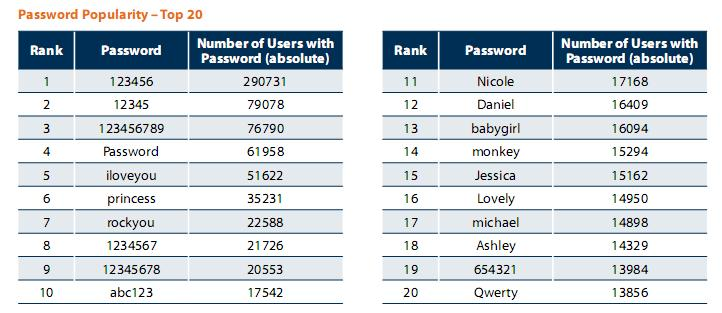
\includegraphics[width=0.8\textwidth]{popular-password.jpg}
    \caption{Most popular passwords from the RockYou}
    \label{fig:pop}
\end{figure}

\bigskip

\item 
I would say that password is "weak" if a person with some amount of logic can come up with this word/combination once he will think a bit (like using your name, service name, etc.). Also, for now, it will be weak if it is somewhere in the lists, published online, because everybody can use them for dictionary attacks. Of course it is weak if it is short or does contain only letters - then it is easy to break it with brute force. I personally do not like randomly generated passwords, that are long, contain lots of numbers, symbols and different case letters - no normal human is able to remember it and of course it will be written down somewhere and definitely attackers will be able to access it sooner or later. Strongest passwords in my opinion are the ones, that have some sense in it, so author can easily remember it, also it has to contain at least numbers and different case of letters - or if it has symbols it can be shorter.

\bigskip

\item Nope =)
\end{itemize}
\subsection*{b) Brute-Force Attacks}
Brute-Force attack is based on guessing as well as dictionary attack. However, it tries \textit{all the possible combinations}. So, if we have
\begin{itemize}
\item $n$ - password length
\item $U$ - set of uppercase letters
\item $L$ - set of lowercase letters
\item $D$ - set of digits
\item $S$ - set of special characters
\end{itemize}
In worst case password will contain elements from all the sets:
$$P=U \cup L \cup D \cup S$$
As all sets are disjunct (their intersection is $\emptyset$):
$$|P|=|U|+|L|+|D|+|S|$$
then in worst case number of possible passwords is $$NUM\_OF\_PSSWDS=|P|^n$$
Increase of $n$ (e.g. with respect to time $t$) will cause faster growth of $NUM\_OF\_PSSWDS$ then increase of $|P|$, because
\begin{itemize}
\item if $P$ fixed, than $NUM\_OF\_PSSWDS=const^{n(t)}$ - exponential growth
\item if $n$ fixed, than $NUM\_OF\_PSSWDS=|P(t)|^{const}$ - polynomial growth 
\end{itemize}
And we know that exponent grows faster than polynomial.

\section*{Task 2.5 (theoretical): PCAP Analysis 1}
\begin{itemize}
\item trace file contains capture of packages traveling over the network
\item the target is DB, used by web application "Dumn Vulnerable Web App" on host 192.168.10.10 ("http://vulnerabilities/sqli") (attacker (192.168.10.1) and attacked host are in the same LAN)
\item attacker commits SQL injection. Steps:
\begin{enumerate}
\item gets web app html page (packages: 4-8)
\item tries to get $id=0$ using form (form's $action=GET$), gets nothing (packages: 10-13)
\item tries to get $id=1$, succeeds (packages: 15-18)
\item gets list of all users by submitting to the form an expression that will be true for all the users: GET ... ?id=1 or 1=1 (packages: 27-31)
\item tries to write sql injection using \textit {union} and \textit{select}, fails and get some hints from error message in response how to proceed further (packages: 40-42) 
\item rewrites sql injection which still do not give any useful results but shows itself as correct one (packages: 51-55)
\item rewrites sql injection from previous step in order to access field \textit{pass}, fails as this field does not exist (packages: 64-66)
\item gets with sqli names of table columns, correct one is \textit{password} (packages: 75-79)
\item rewrites sqli from previous steps to obtain \textit{surname:password} combinations (packages: 88-92)
\item succeeds (packages: 92)
\end{enumerate}
\item form does not have any input field checks that can prevent user from submitting via form some malicious scripts. Also, escape characters are filtered incorrectly or not filtered at all.
\item attacker gets user-names and passwords combinations, and most probably will use obtained data for further malicious actions, e.g. corruption of users' personal data.
\item in general it was successful. Some of requests did not give proper result because of inappropriate SQL syntax. But on the next steps attacker corrected his previous mistakes.
\item links:\\
\url{https://tools.cisco.com/security/center/content/CiscoSecurityAdvisory/cisco-sa-20160203-ucm}\\
\url{http://seclists.org/fulldisclosure/2016/Apr/5}
\item input from the user can be checked with respect to length and content, for example, using Javascript regular expressions. Also some escape characters filter should be provided.
\end{itemize}
\end{document} 
